\end{multicols}

\mysection{Bestiary}{monster-list}


\mysubsection{Adventurers as Monsters}{player-versus-player}


You may encounter a situation where two (or more) Adventurers wish to engage in Combat with one another; alternately, you may wish to stat an Adventurer of your own, and sic them on the Band.  

Simply switch all \RO tries to \RB tries, change levels to Weakness using the Basic Monster table above, and let the dice fall where they may.

\example {  El Ravager (a Sellsword) (Level 6) and Knuckles the Thief (Level 7) decide they've had enough of one another, and throw down.  El Rav's Weakness is d12 and Knuckles Weakness is d10.  Both roll their Init; El Rav rolls a 14 while Knuckles rolls a 12.  Knuckles decides to "bump" his roll by rolling his Luck die, and gets a 4 - making his roll a 16.  He goes first (though El Rav could retaliate by rolling his \TAL, for instance).

\myskip

Knuckles tries his Attack and El Rav tries his Guard.  After rolling various dice (Deed Dice, Luck Dice, Personality, etc)  Knuckles ends up with a 27 and El Rav rolls a 25.  El Rav takes the 12 damage Knuckles rolled to his Grit, then moves in for the kill ...

}

\begin{center}
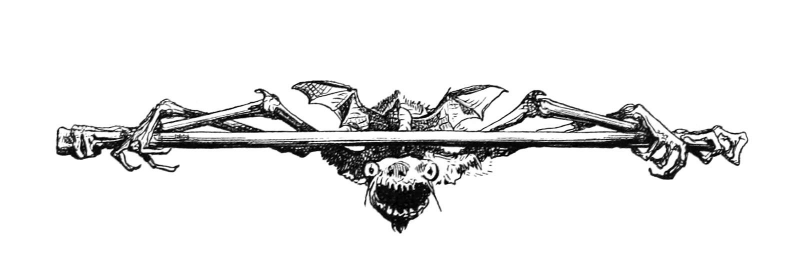
\includegraphics{monsters/Flavor_5}
\end{center}
\newpage



% MONSTERS BEGIN


\mysubsection{Aberrations}{monster-order-aberrations-detail}
\begin{multicols}{2}\raggedbottom




\MONSTER[
  NM=Otyugh,
  LK=monster-otyugh,
  SPD=Base,
  AT=2d8 1 Close AND d8 2 Nearby (Different),
  WK=d10,
  HD=7,
  PR=Average,
  SK=0,
  MR=Orderly,
  SV=5,
  SPL=0,
  TRT=\mytrait{Alien}{monster-trait-alien}; \mytrait{Canny}{monster-trait-canny},
  ACT=\mytrait{Grapple}{monster-action-grapple}
  ]

If you're a Philosopher exploring eldritch blood magics, you're going to generate a lot of trash.  Failed experiments.  Leftover parts.  Weird glowing stones that you figure you probably shouldn't dump into the town water supply.  At some point, someone had the brilliant idea to breed something that could get rid of all that waste; sadly, he or she was probably killed by their creation before it escaped their laboratory.  Otyugh breed prolifically (the details are vague) in carrion, gong fields, and garbage pits.  It's a good idea to keep them well fed, though, lest they start to get hungry ...

The Otyugh attacks 2 Close or Nearby Adventurers with its tentacles, and 1 Close  Adventurer with its bite.  \RBTRY{\VIG}{\VIG} if you are struck with a tentacle or become Grappled.  The Otyugh bite automatically hits a Grappled Adventurer.

\begin{center}
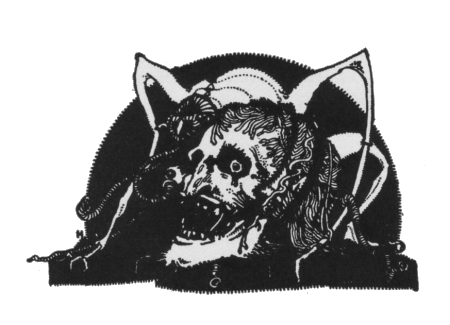
\includegraphics{monsters/Abberation}
\end{center}


\cbreak

\MONSTER[
  NM=Owl Bear,
  LK=monster-owl-bear,
  SPD=Base,
  AT=d6+d8 1 Close,
  WK=d12,
  HD=5,
  PR=Strong,
  SK=0,
  MR=Fanatical,
  SV=7,
  SPL=0,
  TRT=\mytrait{Alien}{monster-trait-alien}; \mytrait{Canny}{monster-trait-canny}; \mytrait{Strong}{monster-trait-strong}; \mytrait{Bloodthirsty}{monster-trait-bloodthirsty},
  ACT=\mytrait{Rage}{monster-action-rage}
  ]
\callout{
    Owlbears roll a d12 for \VIG tries.
}
At some point some Philosopher figured that breeding an owl with a bear would be a really great idea.  They weren't entirely wrong - Owlbears make great guardians and security systems, but they're really, really bad companions and pets.  Nevertheless, Owlbear eggs are worth a great deal to Philosophers who want to train them for their own laboratories (they have about a 20\% success rate, with the other 80\% either not being viable or killing and maiming their "masters").





\MONSTER[
  NM=Priest of Syrinx,
  LK=monster-priest-of-syrinx,
  SPD=Base,
  AT=see below,
  WK=d12,
  HD=5,
  PR=Weak,
  SK=0,
  MR=Cowardly,
  SV=7,
  SPL=4d4,
  TRT=\mytrait{Alien}{monster-trait-alien}; \mytrait{Canny}{monster-trait-canny}; \mytrait{Supportive}{monster-trait-supportive},
  ACT=None
 ]
\callout{

    Priests of Syrinx are immune to \mypg{Secrets of the Mind}{arcana-wizardry-secrets}.

    \hrulefill

    Priests of Syrinx have limited telepathy.  \mybold{Murder} attempts will not work on them, and they can see Invisible creatures.
}

Strange cephalopod headed creatures from some place among the stars.  They speak an alien language that no one has yet been able to decipher (possibly the key rests in the limited telepathy they appear to share).  Priests of Syrinx worship a supremely logical and utterly evil alien intelligence.

In addition to their spells, Priests of Syrinx wield Possibility Swords - blades of psionic energy that collapse possibilities to a single point.  At the top of the Moment, roll 3d6.  You may use any combination of these dice to either reduce physical damage by the amount shown on the die, or deal damage to up to 3 Close Adventurers.   The blade strikes automatically and cannot be Guarded.  

\example {
   At the top of the Moment, you roll 3d6 with a result of 6, 5, 1.  A Sellsword Adventurer wins Init and strikes, hitting for 7 points of damage.  You use the 6 to reduce this damage to 1.  On your turn, you strike back at the Adventurer for 6 (5+1) damage - you could also have split the attack between the Sellsword and one of her compatriots (5 points on one and 1 point on the other)
}

The Possibility Sword requires whatever limited telepathy the Priests of Syrinx possess in order to work correctly.


\MONSTER[
  NM=Rust Monster,
  LK=monster-rust-monster,
  SPD=Base,
  AT=d4 1 Close,
  WK=d20,
  HD=3,
  PR=Average,
  SK=d4,
  MR=Orderly,
  SV=9,
  SPL=0,
  TRT=\mytrait{Alien}{monster-trait-alien}; \mytrait{Canny}{monster-trait-canny},
  ACT=None
 ]
Also known as the "Philosopher's Friend", created and bred to level the playing field.  If an Adventurer with Medium or Heavy armor is struck by a Rust Monster, immediately roll the Armor's \UD \mybold{before} attempting to absorb the attack.  If a Rust Monster is struck by an iron weapon, treat the weapon's damage as a \UD (in other words, move the weapon's damage die \DCDOWN if a 1 or a 2 is rolled).


\MONSTER[
  NM=Son of Kyuss,
  LK=monster-son-of-kyuss,
  SPD=Base,
  AT=2d8 1 Close,
  WK=d8,
  HD=8,
  PR=Average,
  SK=0,
  MR=Orderly,
  SV=4,
  SPL=0,
  TRT=\mytrait{Alien}{monster-trait-alien}; \mytrait{Canny}{monster-trait-canny},
  ACT=None
 ]
Hailing from the void between the stars, the Sons of Kyuss are fanatically racist Monsters bent on the genocide of every last person in Ygg that is not a Son of Kyuss.  The Sons appear as floating orbs with 6 eyestalks and a gigantic maw.

In addition to their ferocious bite, the Sons of Kyuss possess 6 eyestalks that appear to be created from pure Chaos.  The eyes act independently of the body. An eye can be cut off with a successful \mypg{Gambit}{combat-deeds-gambit} each Moment (roll a d6 and remove that eye.  If the Adventurer wants to \mybold{choose} the eye, they get a -4 penalty on their Gambit rolls).  

Because of their Chaotic nature, the eyes are unreliable.  At the top of the Moment, roll a d6 - these are the number of eyes that have been "activated" this Moment.  The eyes are activated in order.  If the eye has been injured or removed, it "counts" towards the total.  For example, if you roll a 4 but the 2nd eye has been removed, then only the 1st, 3rd, and 4th eyes activate.

        \mybold{1st: Ray of Sleep} ~\\ \SAVE{Hex} or be \effect{Slept} for \DUR{d8}.

        \mybold{2nd: Ray of Agony} ~\\ \SAVE{Hex} or take 2d6 damage.

        \mybold{3rd: Ray of Teleportation} ~\\ \SAVE{Hex} or be teleported 1 range (Close to Nearby, Nearby to Far Away) in a random direction.
        
        \mybold{4th: Ray of Weakness} ~\\ \SAVE{Doom} or drop all facets of your \mybold{Personality} \DCDOWN.

        \mybold{5th: Ray of Petrifaction} ~\\ \SAVE{Doom} or be \effect{Paralyzed} for \DUR{d8}.

        \mybold{6th: Ray of Death} ~\\ \SAVE{Doom} or bring your Flesh to 0.  You are dying.  Immediately roll your \DEATH.


\newpage

\mysubsection{Amphibians}{monster-order-amphibians-detail}



\MONSTER[
  NM=Giant Toad,
  LK=monster-giant-toad,
  SPD=Base,
  AT=d6 1 Close,
  WK=d24,
  HD=1,
  PR=Average,
  SK=d4,
  MR=Orderly,
  SV=11,
  SPL=0,
  TRT=\mytrait{Zoological}{monster-trait-zoological}; \mytrait{Slippery}{monster-trait-slippery}; \mytrait{Amphibious}{monster-trait-amphibious}; \mytrait{Leaping}{monster-trait-leaping},
  ACT=\mytrait{Charge}{monster-action-charge}
  ]
\callout{
    2-in-6 chance the Toad has the \mytrait{Venomous}{monster-trait-venomous} Trait.
}
Big-ass toads and frogs; you can usually hear them before you see them.  Have a habit of trying to swallow things whole (including Adventurers).



\MONSTER[
  NM=Salamander,
  LK=monster-salamander,
  SPD=Base,
  AT=d6+d8 1 Close,
  WK=d12,
  HD=5,
  PR=Strong,
  SK=0,
  MR=Orderly,
  SV=7,
  SPL=0,
  TRT=\mytrait{Zoological}{monster-trait-zoological}; \mytrait{Slippery}{monster-trait-slippery}; \mytrait{Amphibious}{monster-trait-amphibious},
  ACT=None
 ]
\callout{
    Immune to damage from fire.

    \hrulefill

    Weak to damage from ice or cold (+2 damage per die).
}

Salamanders ride the coat-tails of Fire, Blood, and Smoke elementals, slithering through the open gates when those creatures are summoned.  They make their homes in bonfires, lava pits, endlessly burning cauldrons, and mystical forges.  Salamanders are classified as Amphibians but instead of being able to breathe and live in water, they can breathe and live in fire.  

If the Salamander is near death or is feeling spiteful, it can explode in a torrent of flame.  Everything Close or Nearby takes 3d6 damage (\SAVE{Doom} for half) and flammable things are set alight.  Makes a big noise.  Covers everyone is Salamander parts.  Also kills the Salamander.

\begin{center}
\myimage{monsters/Toad_Man}
\end{center}

\MONSTER[
  NM=Toad Man,
  LK=monster-toad-man,
  SPD=Base,
  AT=weapon OR d4 / 1 Close,
  WK=d20,
  HD=3,
  PR=Average,
  SK=0,
  MR=Orderly,
  SV=9,
  SPL=0,
  TRT=\mytrait{Zoological}{monster-trait-zoological}; \mytrait{Slippery}{monster-trait-slippery}; \mytrait{Amphibious}{monster-trait-amphibious}; \mytrait{Canny}{monster-trait-canny}; \mytrait{Leaping}{monster-trait-leaping},
  ACT=\mytrait{Charge}{monster-action-charge}
  ]
Hilarious looking half-man, half-toad bipeds. Almost impossible to take seriously, except for the fact that they are armed and have no sense of humor. They prefer spears to make the best use of their leaping attacks.


\MONSTER[
  NM=Troglodyte,
  LK=monster-troglodyte,
  SPD=Base,
  AT=weapon OR d6 / 1 Close,
  WK=d24,
  HD=1,
  PR=Average,
  SK=0,
  MR=Orderly,
  SV=11,
  SPL=0,
  TRT=\mytrait{Zoological}{monster-trait-zoological}; \mytrait{Slippery}{monster-trait-slippery}; \mytrait{Amphibious}{monster-trait-amphibious}; \mytrait{Nocturnal}{monster-trait-nocturnal},
  ACT=None
 ]
Bipedal dwellers of caves and caverns, thought to be rejects from the \mybold{Veins of the Earth}, a confusing mix of salamander and toad.  Trogs can spend an Action emitting a foul smelling gas that causes \effect{Disgust} to Adventurers who are Close unless they \SAVE{Toxins}.  The smell lasts for Minutes.



\newpage
\mysubsection{Arthropods}{monster-order-arthropods-detail}




\MONSTER[
  NM=Giant Ant,
  LK=monster-giant-ant,
  SPD=Base,
  AT=d10 1 Close,
  WK=d20,
  HD=3,
  PR=Average,
  SK=d4,
  MR=Orderly,
  SV=9,
  SPL=0,
  TRT=\mytrait{Zoological}{monster-trait-zoological}; \mytrait{Pack}{monster-trait-pack},
  ACT=None
 ]
\callout{
    Giants Ants have Fanatical morale when defending their homes.
}

\ed{Have you seen the movie "Them!" (1954) by any chance?  It's got Edmund Gwenn, the guy who plays Santa Claus in Capra's "Miracle on 34th Street".   You should check it out.}

Even normal ants have all kinds of ways of ruining your life.  If you feel your Adventurers are under-challenged, roll a d6 - the Giant Ant has:

\mynumlist {
    \item the \mytrait{Venomous}{monster-trait-venomous} Trait.
    \item the \mytrait{Acidic}{monster-trait-acidic} Trait.
    \item the \mytrait{Flying}{monster-trait-flying} Trait.
    \item a paralytic bite. \SAVE{Toxins} if the Monster hits Flesh or be \effect{Paralyzed} for \DUR{d4}.
    \item a stinger, can attack d10 2 Close (Either).
    \item the \mytrait{Frenzied}{monster-trait-frenzied} Trait.
} 


\MONSTER[
  NM=Giant Beetle,
  LK=monster-giant-beetle,
  SPD=Slow,
  AT=d6+d8 1 Close,
  WK=d20,
  HD=5,
  PR=Strong,
  SK=d6,
  MR=Orderly,
  SV=7,
  SPL=0,
  TRT=\mytrait{Zoological}{monster-trait-zoological},
  ACT=None
 ]
Boring beetles.  Deathwatch beetles.  Carrion beetles.  Long-horned beetles.  Predacious diving beetles.  Pleasing fungus beetles!  SOLDIER BEETLES!  No shit, there are even spider beetles (\myital{Anobiidae}). Long and short, use these stats as a base, but hit wikipedia.



\MONSTER[
  NM=Giant Centipede,
  LK=monster-giant-centipede,
  SPD=Fast,
  AT=d6 1 Close AND 1 dmg d6 Close (Either),
  WK=d16,
  HD=4,
  PR=Average,
  SK=0,
  MR=Orderly,
  SV=8,
  SPL=0,
  TRT=\mytrait{Zoological}{monster-trait-zoological}; \mytrait{Venomous}{monster-trait-venomous}; \mytrait{Twitchy}{monster-trait-twitchy},
  ACT=None
 ]

\callout{
    Giant Centipede roll a d12 for \DEX tries.
}
Really fast giant crawling insects with far too many legs.   Makes a hissing sound as it flies down a tunnel to consume an Adventurer.

At the top of the Moment, roll a d6 - the Centipede can attack with this many legs in addition to gnawing with its horrific mouth parts. The legs only deal 1 point of damage, but they are also \mytrait{Venomous}{monster-trait-venomous}.

\myimage{monsters/Arthropods}

\MONSTER[
  NM=Giant Spider,
  LK=monster-giant-spider,
  SPD=Fast,
  AT=d8 1 Nearby,
  WK=d20,
  HD=2,
  PR=Average,
  SK=0,
  MR=Orderly,
  SV=10,
  SPL=d4,
  TRT=\mytrait{Zoological}{monster-trait-zoological}; \mytrait{Venomous}{monster-trait-venomous},
  ACT=None
 ]
I mean ... it's a giant goddamn spider, anywhere between the size of a mastiff to the size of small van (increase \HD accordingly).  

Giant Spiders can use their Spell die to cast the \mypg{Secret: Web}{secrets-web} (only). 




\newpage

\mysubsection{Automatons}{monster-order-automatons-detail}


\MONSTER[
  NM=Iron Serpent,
  LK=monster-iron-serpent,
  SPD=Fast,
  AT=2d8 2 Close (Either),
  WK=d10,
  HD=7,
  PR=Average,
  SK=d8,
  MR=n/a,
  SV=5,
  SPL=0,
  TRT=\mytrait{Mindless}{monster-trait-mindless}; \mytrait{Unhallowed}{monster-trait-unhallowed}; \mytrait{Twitchy}{monster-trait-twitchy},
  ACT=None
 ]

\callout{
    Iron Serpents roll a d12 for \DEX tries.
}

5 or 6 meter long serpents made of iron and Faith, usually set to guard tombs, shrines, or altars.  Extremely tough and greatly feared.  They are known to pursue intruders tirelessly until they are destroyed; unscrupulous Bands will send in linkboys, meat shields, and villagers to attract their attention ...

If an Iron Serpent strikes Flesh, the victim must \SAVE{Hexes};  Failure means a roll on the \mypg{Lesser Curses}{table-lesser-curses} table.




\MONSTER[
  NM=Living Statue,
  LK=monster-living-statue,
  SPD=Slow,
  AT=2d6 2 Close (Combined),
  WK=d12,
  HD=5,
  PR=Strong,
  SK=d8,
  MR=n/a,
  SV=7,
  SPL=0,
  TRT=\mytrait{Mindless}{monster-trait-mindless}; \mytrait{Unhallowed}{monster-trait-unhallowed}; \mytrait{Strong}{monster-trait-strong},
  ACT=\mytrait{Throw}{monster-action-throw}
  ]

\callout{
    Living Statues roll a d12 for \VIG tries.
}

Caryatids, maquettes, falla, and effigies; not quite \mypg{Golems}{miracle-golem}, but almost as powerful.  Often set to guard entrances, and mixed in with other (normal) statues of the same type.  Philosophers often place a \mypg{Talking Sigil}{inscription-sigil-talking}  on them, usually to shout out that there are intruders wandering about.

Living Statues can \mytrait{Throw}{monster-action-throw} an Adventurer 20m.

\cbreak

\vspace*{5mm}

\MONSTER[
  NM=Robot,
  LK=monster-robot,
  SPD=Base,
  AT=d8 1 Nearby,
  WK=d20,
  HD=3,
  PR=Average,
  SK=d8,
  MR=n/a,
  SV=9,
  SPL=0,
  TRT=\mytrait{Mindless}{monster-trait-mindless}; \mytrait{Unhallowed}{monster-trait-unhallowed}; \mytrait{Supportive}{monster-trait-supportive}; \mytrait{Militant}{monster-trait-militant},
  ACT=None
 ]
Metal creatures of unknown provenance, of various heights and sizes.  They always appear in geometric binary sequences (2,4,8,16,etc).


\begin{center}

\includegraphics{monsters/MonsterAutomaton}
\end{center}

\newpage
\mysubsection{Demons}{monster-order-demons-detail}

\MONSTER[
  NM=Ba'al,
  LK=monster-baal,
  SPD=Base,
  AT=d6+d8 1 Close,
  WK=d16,
  HD=5,
  PR=Average,
  SK=0,
  MR=Orderly,
  SV=7,
  SPL=0,
  TRT=\mytrait{Unhallowed}{monster-trait-unhallowed}; \mytrait{Terrifying}{monster-trait-terrifying}; \mytrait{Chaotic}{monster-trait-chaotic}; \mytrait{Nocturnal}{monster-trait-nocturnal}; \mytrait{Otherworldly}{monster-trait-otherworldly}; \mytrait{Strong}{monster-trait-strong}; \mytrait{Slippery}{monster-trait-slippery}; \mytrait{Leaping}{monster-trait-leaping},
  ACT=\mytrait{Charge}{monster-action-charge}; \mytrait{Rage}{monster-action-rage}
  ]
\callout{
    Ba'al roll a d12 for \VIG tries.
}

Powerful toad-demons who appear to have some sort of military structure that only they truly understand.  They have command over creatures of the \mybold{Amphibian} Order, who use them as pawns or mounts.



\MONSTER[
  NM=Dretch,
  LK=monster-dretch,
  SPD=Base,
  AT=d6 1 Close,
  WK=d24,
  HD=1,
  PR=Weak,
  SK=0,
  MR=Cowardly,
  SV=11,
  SPL=0,
  TRT=\mytrait{Unhallowed}{monster-trait-unhallowed}; \mytrait{Terrifying}{monster-trait-terrifying}; \mytrait{Chaotic}{monster-trait-chaotic}; \mytrait{Nocturnal}{monster-trait-nocturnal}; \mytrait{Otherworldly}{monster-trait-otherworldly}; \mytrait{Pack}{monster-trait-pack}; \mytrait{Stupid}{monster-trait-stupid},
  ACT=None
 ]
The lowest of demonkind, fodder for their constant battles.  Created from the cast off souls of Mortals in mockery of \TheAuthority.  Extremely stupid and possessing extraordinarily low self esteem.


\cbreak

\vspace*{5mm}

\MONSTER[
  NM=Naga,
  LK=monster-naga,
  SPD=Fast,
  AT=see below,
  WK=d10,
  HD=7,
  PR=Average,
  SK=d8,
  MR=Fanatical,
  SV=5,
  SPL=0,
  TRT=\mytrait{Unhallowed}{monster-trait-unhallowed}; \mytrait{Terrifying}{monster-trait-terrifying}; \mytrait{Chaotic}{monster-trait-chaotic}; \mytrait{Nocturnal}{monster-trait-nocturnal}; \mytrait{Otherworldly}{monster-trait-otherworldly},
  ACT=None
 ]
\callout{
    Naga roll a d12 for \DEX tries.
}
Multi-armed half-snake, half Mortal demons, second only to Pit Fiends in power.  Fast, clever, and depraved.  They wield blades made of shadow in each of their hands, which blink in and out of existence.


At the top of each Moment, roll a d8.  The Naga is able to attack up to \SUM Close Adventurers (Either); each blade deals \SUM damage.  Note that the Naga can concentrate all of its attacks on a single hapless Adventurer if it so chooses.

\myimage{monsters/MonsterNaga}

\newpage

\end{multicols*}
\myimage{monsters/Demon2}
\begin{multicols*}{2}


\MONSTER[
  NM=Pit Fiend,
  LK=monster-pit-fiend,
  SPD=Base,
  AT=d24+d4 / 1d8 1 Close +1 Nearby,
  WK=d4,
  HD=9,
  PR=Strong,
  SK=d10,
  MR=n/a,
  SV=3,
  SPL=0,
  TRT=\mytrait{Unhallowed}{monster-trait-unhallowed}; \mytrait{Terrifying}{monster-trait-terrifying}; \mytrait{Chaotic}{monster-trait-chaotic}; \mytrait{Nocturnal}{monster-trait-nocturnal}; \mytrait{Otherworldly}{monster-trait-otherworldly},
  ACT=\mytrait{Rage}{monster-action-rage}; \mytrait{Trample}{monster-action-trample}
  ]

I hope you saw The Fellowship of the Ring in the theaters, but maybe you were too young.  First time I saw the Balrog pop out to give Gandalf a run for his money, I actually spilled my popcorn.  The Pit Fiend is similar - just a giant, depraved, utterly evil, terrifying winged monster from the 9th plane of Hell.

The Pit Fiend strikes Close Adventurers with an abyssal blade (d24+4) that also deals \mypg{Rending}{weapon-attribute-rending} damage.  If an Adventurer is struck with the demon's whip (d8 Close or Nearby), they must \RBTRY{\DEX}{\VIG} or be immediately dragged to Close range.  The Pit Fiend can combine these into one Combat Maneuver if it wants i.e. hit an Adventurer with its whip and then strike with it sword.

Finally, Adventurers (and other Monsters) Close to the Pit Fiend must contend with its abyssal flames.  These flames deal d6 damage at the bottom of every Moment unless a \SAVE{Doom} try is made.








\MONSTER[
  NM=Vrock,
  LK=monster-vrock,
  SPD=Base,
  AT=2d6 2 Close (Combined),
  WK=d20,
  HD=3,
  PR=Average,
  SK=0,
  MR=Cowardly,
  SV=9,
  SPL=0,
  TRT=\mytrait{Unhallowed}{monster-trait-unhallowed}; \mytrait{Terrifying}{monster-trait-terrifying}; \mytrait{Chaotic}{monster-trait-chaotic}; \mytrait{Nocturnal}{monster-trait-nocturnal}; \mytrait{Otherworldly}{monster-trait-otherworldly}; \mytrait{Canny}{monster-trait-canny}; \mytrait{Bloodthirsty}{monster-trait-bloodthirsty}; \mytrait{Flying}{monster-trait-flying},
  ACT=None
 ]
A winged biped with the head of a toothed vulture and the talons of a raptor; extremely opportunistic, cowardly, and unpleasant.  While they have the \mytrait{Flying}{monster-trait-flying} trait, they are really bad at it and require 2 Actions to move 1 range step.

\newpage


\mysubsection{Dinosaurs}{monster-order-dinosaurs-detail}


\MONSTER[
  NM=Allosaurus,
  LK=monster-allosaurus,
  SPD=Fast,
  AT=2d8 1 Close,
  WK=d12,
  HD=6,
  PR=Average,
  SK=d6,
  MR=Cowardly,
  SV=6,
  SPL=0,
  TRT=\mytrait{Terrifying}{monster-trait-terrifying}; \mytrait{Zoological}{monster-trait-zoological}; \mytrait{Frenzied}{monster-trait-frenzied}; \mytrait{Twitchy}{monster-trait-twitchy},
  ACT=None
 ]

\callout{
    Allosaurus roll a d12 for \DEX tries.
}
7.5 to 10.5 meter long, 1800kg bipedal theropod.  Like a T-Rex but juuuust a little smaller.




\MONSTER[
  NM=Plesiosarus,
  LK=monster-plesiosarus,
  SPD=Base,
  AT=d20 1 Close,
  WK=d10,
  HD=7,
  PR=Average,
  SK=d6,
  MR=Cowardly,
  SV=5,
  SPL=0,
  TRT=\mytrait{Terrifying}{monster-trait-terrifying}; \mytrait{Zoological}{monster-trait-zoological}; \mytrait{Frenzied}{monster-trait-frenzied},
  ACT=None
 ]
5m long, 450kg marine dinosaur. They prefer warm waters, and can swim two ranges in a single Action.

\myimage{monsters/MonsterTrex}

\cbreak

\MONSTER[
  NM=Pteranodon,
  LK=monster-pteranodon,
  SPD=Base,
  AT=2d6 1 Close,
  WK=d16,
  HD=5,
  PR=Average,
  SK=0,
  MR=Cowardly,
  SV=7,
  SPL=0,
  TRT=\mytrait{Terrifying}{monster-trait-terrifying}; \mytrait{Zoological}{monster-trait-zoological}; \mytrait{Frenzied}{monster-trait-frenzied}; \mytrait{Flying}{monster-trait-flying},
  ACT=None
 ]
Clumsy flying dinosaurs with a 6-7 meter wingspan, can easily pick up something 100kg or less in its talons to drop it from a height, or attack with its snapping maw.


\MONSTER[
  NM=Triceratops,
  LK=monster-triceratops,
  SPD=Base,
  AT=2d8 1 Close,
  WK=d12,
  HD=6,
  PR=Strong,
  SK=d10,
  MR=Cowardly,
  SV=6,
  SPL=0,
  TRT=\mytrait{Terrifying}{monster-trait-terrifying}; \mytrait{Zoological}{monster-trait-zoological}; \mytrait{Frenzied}{monster-trait-frenzied},
  ACT=\mytrait{Trample}{monster-action-trample}
  ]
Quadrupedal dinosaur about 9m long and weighing a ridiculous 12 metric tons.  Generally pretty peaceful but short tempered if you decide to fuck with it (think rhinoceros but ... you know, a lot bigger).

Gores with its horns for 2d8 damage, but prefers to charge if it can.  If the Triceratops is able to move from Nearby to Close without taking damage, it will deal \MAX damage (16 points), and the unlucky Adventurer is knocked \effect{Prone} unless they can \RBTRY{\VIG}{\VIG}.


\MONSTER[
  NM=Tyrannosaurus Rex,
  LK=monster-tyrannosaurus-rex,
  SPD=Base,
  AT=d24+4 1 Close,
  WK=d8,
  HD=8,
  PR=Strong,
  SK=d10,
  MR=n/a,
  SV=4,
  SPL=0,
  TRT=\mytrait{Terrifying}{monster-trait-terrifying}; \mytrait{Zoological}{monster-trait-zoological}; \mytrait{Frenzied}{monster-trait-frenzied},
  ACT=\mytrait{Rage}{monster-action-rage}
  ]
The goddamn king.  If the T-Rex ever rolls \MAX damage, the Adventurer must make a \SAVE{Doom} or be immediately bitten in half.  This kills the Adventurer.

\newpage


\mysubsection{Dire Beasts}{monster-order-dire-beasts-detail}






\MONSTER[
  NM=Cannibal Ape,
  LK=monster-cannibal-ape,
  SPD=Base,
  AT=2d6 1 Close,
  WK=d16,
  HD=4,
  PR=Strong,
  SK=0,
  MR=Orderly,
  SV=8,
  SPL=0,
  TRT=\mytrait{Berserk}{monster-trait-berserk}; \mytrait{Zoological}{monster-trait-zoological}; \mytrait{Cannibal}{monster-trait-cannibal},
  ACT=\mytrait{Rage}{monster-action-rage}
  ]


\callout{
    Cannibal Apes roll a d12 for \VIG tries.
}
Favorite monster of Conan and other barbarian lit, fond of ripping creatures limb from limb and feasting on them while they're still alive and fresh.




\MONSTER[
  NM=Cave Bear,
  LK=monster-cave-bear,
  SPD=Slow,
  AT=2d6 1 Close AND d10 dmg 2 Close (Either),
  WK=d16,
  HD=5,
  PR=Strong,
  SK=d4,
  MR=Fanatical,
  SV=7,
  SPL=0,
  TRT=\mytrait{Berserk}{monster-trait-berserk}; \mytrait{Zoological}{monster-trait-zoological}; \mytrait{Strong}{monster-trait-strong},
  ACT=\mytrait{Charge}{monster-action-charge}
  ]
\callout{
    Cave Bears roll a d12 for \VIG tries.
}
3.5 meter long and 1,000kg of pure killing machine.  The Cave Bear can concentrate all 3 attacks on a single hapless Adventurer, or its bite (2d6) on one and claws (d10 / d10) on another.

\myimage{monsters/MonsterSabertooth}


\cbreak

\myimage{monsters/MonsterCaveBear}

\MONSTER[
  NM=Dire Wolf,
  LK=monster-dire-wolf,
  SPD=Fast,
  AT=d8 1 Close,
  WK=d20,
  HD=3,
  PR=Average,
  SK=0,
  MR=Orderly,
  SV=9,
  SPL=0,
  TRT=\mytrait{Berserk}{monster-trait-berserk}; \mytrait{Zoological}{monster-trait-zoological}; \mytrait{Pack}{monster-trait-pack},
  ACT=None
 ]
2m long and 50kg, these killers like to hunt in packs.  Smarter than you think, they'll work together in ways Adventurers might not anticipate.

\MONSTER[
  NM=Sabertooth Cat,
  LK=monster-sabertooth-cat,
  SPD=Base,
  AT=d6+d8 1 Close AND 2d6 dmg 2 Close (Either),
  WK=d12,
  HD=6,
  PR=Average,
  SK=0,
  MR=Fanatical,
  SV=6,
  SPL=0,
  TRT=\mytrait{Berserk}{monster-trait-berserk}; \mytrait{Zoological}{monster-trait-zoological}; \mytrait{Frenzied}{monster-trait-frenzied}; \mytrait{Bloodthirsty}{monster-trait-bloodthirsty},
  ACT=None
 ]
King of the Dire Beasts, weighing in at 450kg and standing 1.2m at the shoulder.  The Sabertooth Cat can concentrate all 3 attacks on a single hapless Adventurer, or its bite (d6+d8) on one and claws (2d6) on another.  If both claws hit, the attack also \mypg{Rends}{weapon-attribute-rending}.



\newpage
\mysubsection{Giantkin}{monster-order-giantkin-detail}




\MONSTER[
  NM=Giant,
  LK=monster-giant,
  SPD=Slow,
  AT=d20 All Close (Distinct) OR see below,
  WK=d8,
  HD=8,
  PR=Strong,
  SK=0,
  MR=Cowardly,
  SV=4,
  SPL=0,
  TRT=\mytrait{Strong}{monster-trait-strong}; \mytrait{Stupid}{monster-trait-stupid},
  ACT=\mytrait{Throw}{monster-action-throw}
  ]

\callout{
    Giants roll a d16 for \VIG tries.
}

Massive (4-6m tall) bipedal humanoids.  Giants prefer to fight with giant tree-trunks, massive broken stalagmites, dragon-bones etc. with giant (haha!) sweeping attacks, as well as kicking and stomping with their feet.  If an Adventurer is struck by one of these attacks, they must \RSTRY{\VIG} or be \effect{Stunned} for \DUR{d4}.



In lieu of this sweeping attack, Giants can use one of the following Combat Maneuvers:


\mybullet {
    \item Grab up to d3 Close (Distinct) Adventurers with the \mytrait{Throw}{monster-action-throw} Action to a distance of 30m.
    \item  Grab a large rock, wagon, cow, etc. and toss it somewhere Nearby.  All Adventurers Close to the point of impact must \RS : \VIG or \DEX (Adventurer's Choice) or be \effect{Stunned} for \DUR{d4}.
    \item  Let out a massive roar.  All Adventurers Close to the sound must \SAVE{Doom} or be \effect{Deafened} for \DUR{d4} and must immediately make an \INSANITY try.
    \item  Leap in the air and land with a crash.  All Adventurers Close must \RS : \VIG or \DEX (Adventurer's choice) or be knocked \effect{Prone}.
}

\cbreak

\vspace*{20mm}
\myimage{monsters/Giant}

\end{multicols*}
\begin{center}
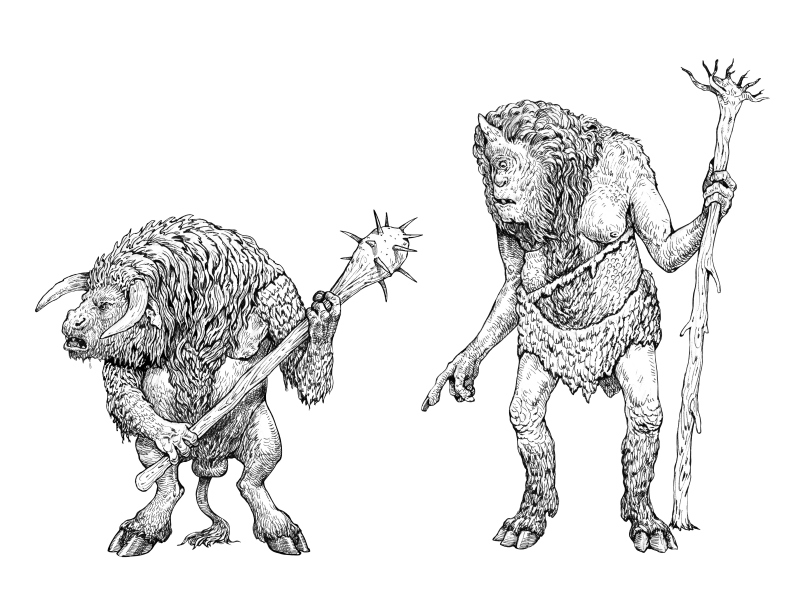
\includegraphics[width=.9\linewidth,keepaspectratio=true]{monsters/MonsterMinotaurOgre}
\end{center}

\begin{multicols*}{2}




\MONSTER[
  NM=Minotaur,
  LK=monster-minotaur,
  SPD=Base,
  AT=2d8 1 Close AND d10 2 Close (Combined),
  WK=d10,
  HD=7,
  PR=Strong,
  SK=0,
  MR=Fanatical,
  SV=5,
  SPL=0,
  TRT=\mytrait{Strong}{monster-trait-strong}; \mytrait{Stupid}{monster-trait-stupid}; \mytrait{Berserk}{monster-trait-berserk},
  ACT=\mytrait{Charge}{monster-action-charge}; \mytrait{Rage}{monster-action-rage}
  ]
\callout{
    Minotaur roll a d12 for \VIG tries.
}
The bovine-headed abominations of myth, usually armed with a giant axe and a bad attitude.   The Minotaur can concentrate all 3 attacks on a single hapless Adventurer, or its axe (2d8) on one and horns (d10 / d10) on another.

\myimage{monsters/Minotaur}




\MONSTER[
  NM=Ogre,
  LK=monster-ogre,
  SPD=Slow,
  AT=2d6 1 Close,
  WK=d16,
  HD=4,
  PR=Strong,
  SK=0,
  MR=Fanatical,
  SV=8,
  SPL=0,
  TRT=\mytrait{Strong}{monster-trait-strong}; \mytrait{Stupid}{monster-trait-stupid}; \mytrait{Bloodthirsty}{monster-trait-bloodthirsty},
  ACT=\mytrait{Throw}{monster-action-throw}
  ]
\callout{
    Ogres roll a d12 for \VIG tries.
}


Smaller cousin of "true" giants, standing roughly 3m tall.  Somehow a whole lot stupider.  In emulation of their big brothers and sisters, they prefer clubs made out of massive tree branch which they use to pulverize their prey (Ogres surprisingly have very weak teeth and can only eat things that are in "paste" form).  1-in-6 ogres have 2 heads, another 1-in-6 have one eye.

Ogres can \mytrait{Throw}{monster-action-throw} an Adventurer 10m.


\MONSTER[
  NM=Troll,
  LK=monster-troll,
  SPD=Base,
  AT=2d6 1 Close,
  WK=d12,
  HD=6,
  PR=Strong,
  SK=0,
  MR=Orderly,
  SV=6,
  SPL=0,
  TRT=\mytrait{Strong}{monster-trait-strong}; \mytrait{Stupid}{monster-trait-stupid}; \mytrait{Nocturnal}{monster-trait-nocturnal},
  ACT=None
 ]
\callout{
Trolls are Cowardly when facing fire.

Trolls heal 3 Health at the bottom of every Moment.
}

\myimage{monsters/Troll}

Green, gray, or blue skinned Monsters that inhabit caves, swamps, and dark forests.  Nasty bits of work, but deeply afraid of fire.

Trolls will heal 3 Health at the bottom of every Moment if the damage source was not fire.  



\MONSTER[
  NM=Wendigo,
  LK=monster-wendigo,
  SPD=Base,
  AT=2d6 1 Close,
  WK=d16,
  HD=5,
  PR=Average,
  SK=0,
  MR=Fanatical,
  SV=7,
  SPL=0,
  TRT=\mytrait{Strong}{monster-trait-strong}; \mytrait{Stupid}{monster-trait-stupid}; \mytrait{Terrifying}{monster-trait-terrifying}; \mytrait{Cannibal}{monster-trait-cannibal},
  ACT=\mytrait{Rage}{monster-action-rage}
  ]
\callout{
    Wendigo roll a d12 for \VIG tries.
}

Malevolent, cannibalistic, and supernatural Monsters usually found in cold regions, or regions where famine is rampant. Descriptions by the famished and insane survivors of Wendigo attacks differ, but generally agree on the form of a tall (2.5m), gaunt beast with long claws, black eyes, and a mouth with too many teeth.


\newpage

\mysubsection{Goblinoids}{monster-order-goblinoids-detail}

\MONSTER[
  NM=Bugbear,
  LK=monster-bugbear,
  SPD=Base,
  AT=d10 1 Close,
  WK=d20,
  HD=3,
  PR=Strong,
  SK=0,
  MR=Fanatical,
  SV=9,
  SPL=0,
  TRT=\mytrait{Nocturnal}{monster-trait-nocturnal}; \mytrait{Canny}{monster-trait-canny}; \mytrait{Bloodthirsty}{monster-trait-bloodthirsty},
  ACT=\mytrait{Rage}{monster-action-rage}
  ]
Giant hairy goblins that attack with iron-hard claws.  If a Bugbear successfully hits an Adventurer, they can \mypg{Rend}{weapon-attribute-rending} instead of dealing damage.  They like to target heavily armored Adventurers and peel them like grapes.




\MONSTER[
  NM=Gnoll,
  LK=monster-gnoll,
  SPD=Fast,
  AT=weapon or d6 / 1 Close,
  WK=d20,
  HD=2,
  PR=Average,
  SK=0,
  MR=Orderly,
  SV=10,
  SPL=0,
  TRT=\mytrait{Nocturnal}{monster-trait-nocturnal}; \mytrait{Canny}{monster-trait-canny}; \mytrait{Pack}{monster-trait-pack}; \mytrait{Militant}{monster-trait-militant},
  ACT=\mytrait{Charge}{monster-action-charge}
  ]
Militant hyena-headed goblinoids that prefer hit-and-run tactics.  They prefer spears and flails for their dirty work.



\MONSTER[
  NM=Goblin,
  LK=monster-goblin,
  SPD=Fast,
  AT=weapon or d4 / 1 Close,
  WK=d24,
  HD=1,
  PR=Weak,
  SK=0,
  MR=Cowardly,
  SV=11,
  SPL=0,
  TRT=\mytrait{Nocturnal}{monster-trait-nocturnal}; \mytrait{Canny}{monster-trait-canny}; \mytrait{Pack}{monster-trait-pack},
  ACT=\mytrait{Charge}{monster-action-charge}; \mytrait{Rout}{monster-action-rout}
  ]
Tiny evil chattering critters that work well together (up to a point) to take down Adventurers.



\MONSTER[
  NM=Hobgoblin,
  LK=monster-hobgoblin,
  SPD=Base,
  AT=weapon 1 Close OR weapon 1 Far-Away (Bow) OR d4 1 Close,
  WK=d24,
  HD=2,
  PR=Average,
  SK=0,
  MR=Orderly,
  SV=10,
  SPL=0,
  TRT=\mytrait{Nocturnal}{monster-trait-nocturnal}; \mytrait{Canny}{monster-trait-canny}; \mytrait{Militant}{monster-trait-militant},
  ACT=\mytrait{Charge}{monster-action-charge}
  ]
Bigger and more militant than the Goblins they lead.   "Hobs" are usually armed with short bows in addition to melee weapons, and if unarmed are still able to strike with their hands and feet for 3 damage.




\MONSTER[
  NM=Kobold,
  LK=monster-kobold,
  SPD=Base,
  AT=d4 1 Close OR d4 1 Nearby,
  WK=d24,
  HD=0,
  PR=Weak,
  SK=0,
  MR=Cowardly,
  SV=12,
  SPL=0,
  TRT=\mytrait{Nocturnal}{monster-trait-nocturnal}; \mytrait{Canny}{monster-trait-canny},
  ACT=\mytrait{Rout}{monster-action-rout}
  ]
Dog-headed tiny critters, about the size of a Pooka.  Kobolds fight with improvised weapons with surprising skill - broken bottles, sacks of rusty nails, rolling pins, sharp sticks, etc  They can throw these weapons in addition to using them in close combat.  Regardless of the weapon, it deals d4 damage.

\myimage{monsters/Kobold}

If they are disarmed or lose their weapon, they may spend an Action to improvise a new one.  





\MONSTER[
  NM=Orc,
  LK=monster-orc,
  SPD=Base,
  AT=d6 1 Close,
  WK=d24,
  HD=1,
  PR=Strong,
  SK=0,
  MR=Fanatical,
  SV=11,
  SPL=0,
  TRT=\mytrait{Nocturnal}{monster-trait-nocturnal}; \mytrait{Canny}{monster-trait-canny}; \mytrait{Cannibal}{monster-trait-cannibal}; \mytrait{Militant}{monster-trait-militant},
  ACT=\mytrait{Charge}{monster-action-charge}
  ]
Pig-faced classics.  Very reliable (to the Arbiter, I mean).  Often stuck guarding chests in 10'x10' rooms.  Always deal d6 damage whether they're armed or not. 

\newpage
\mysubsection{Goos}{monster-order-goos-detail}




\MONSTER[
  NM=Black Jelly,
  LK=monster-black-jelly,
  SPD=Slow,
  AT=d10 1 Close,
  WK=d20,
  HD=3,
  PR=Average,
  SK=0,
  MR=n/a,
  SV=9,
  SPL=0,
  TRT=\mytrait{Mindless}{monster-trait-mindless}; \mytrait{Amorphous}{monster-trait-amorphous}; \mytrait{Splitting}{monster-trait-splitting}; \mytrait{Acidic}{monster-trait-acidic},
  ACT=None
 ]
\callout{
    At the start of every Moment, roll a d3.  The result is the Gelatinous Cube's Soak for that Moment: 1 (d4), 2 (d6). 
}
Big, oily, black, acidic sentient goo.   Cold-based damage dealt to a Black Jelly will not cause it to Split.

\myimage{monsters/Goo_3}


\MONSTER[
  NM=Gelatinous Cube,
  LK=monster-gelatinous-cube,
  SPD=Slow,
  AT=see below,
  WK=d16,
  HD=4,
  PR=Average,
  SK=see below,
  MR=n/a,
  SV=8,
  SPL=0,
  TRT=\mytrait{Mindless}{monster-trait-mindless}; \mytrait{Amorphous}{monster-trait-amorphous}; \mytrait{Splitting}{monster-trait-splitting},
  ACT=None
 ]
\callout{
    At the start of every Moment, roll a d3.  The result is the Gelatinous Cube's Soak for that Moment: 1 (d4), 2 (d6), 3 (d8). 
}
Opaque cube-shaped wandering goos.  

Creatures hit by a Gelatinous Cube are engulfed unless they win a \RB : \VIG or \DEX try (Adventurer choice) vs. the Gelatinous Cube's \VIG.

Engulfed creatures take ongoing d6 damage at the top of every Moment.  It's possible to cut your way out, but Attack \RO tries are made at -4 while engulfed, and damage dealt is -2 (minimum 1).  Spellcasting is impossible while engulfed.

Successful attacks made from inside the Gelatinous Cube will not cause it to Split.


\MONSTER[
  NM=Green Slime,
  LK=monster-green-slime,
  SPD=Slow,
  AT=d8 1 Close,
  WK=d20,
  HD=2,
  PR=Average,
  SK=d4,
  MR=n/a,
  SV=10,
  SPL=0,
  TRT=\mytrait{Mindless}{monster-trait-mindless}; \mytrait{Amorphous}{monster-trait-amorphous}; \mytrait{Splitting}{monster-trait-splitting},
  ACT=None
 ]
Green, sticky, wet, sucking goos.


\MONSTER[
  NM=Ochre Mold,
  LK=monster-ochre-mold,
  SPD=Slow,
  AT=d12 1 Close,
  WK=d16,
  HD=5,
  PR=Average,
  SK=0,
  MR=n/a,
  SV=7,
  SPL=0,
  TRT=\mytrait{Mindless}{monster-trait-mindless}; \mytrait{Amorphous}{monster-trait-amorphous}; \mytrait{Splitting}{monster-trait-splitting}; \mytrait{Venomous}{monster-trait-venomous},
  ACT=None
 ]

\callout{
    At the start of every Moment, roll a d3.  The result is the Gelatinous Cube's Soak for that Moment: 1 (d4), 2 (d6), 3 (d8), 4 (d10). 
}

Toxic orange-yellow furry molds.  Fire-based damage dealt to an Ochre Mold will not cause it to Split.

\newpage
\mysubsection{Horrors}{monster-order-horrors-detail}




\MONSTER[
  NM=Ghast,
  LK=monster-ghast,
  SPD=Base,
  AT=d8 1 Close,
  WK=d16,
  HD=4,
  PR=Average,
  SK=0,
  MR=Orderly,
  SV=8,
  SPL=0,
  TRT=\small{\mytrait{Unhallowed}{monster-trait-unhallowed}; \mytrait{Terrifying}{monster-trait-terrifying}; \mytrait{Nocturnal}{monster-trait-nocturnal}; \mytrait{Bloodthirsty}{monster-trait-bloodthirsty}; \mytrait{Leaping}{monster-trait-leaping}},
  ACT=None
 ]
\flavor{... the ghasts, those repulsive beings which die in the light, and which live in the vaults of Zin and leap on long hind legs like kangaroos ... After a moment something about the size of a small horse hopped out into the grey twilight, and Carter turned sick at the aspect of that scabrous and unwholesome beast, whose face is so curiously human despite the absence of a nose, a forehead, and other important particulars ... \Tilde H.P. Lovecraft }

Strikes from a Ghast are paralytic.  If a Ghast strikes Flesh, the Adventurer must \RS: \FOC\@ - failure means they are \effect{Paralyzed} for \DUR{d4}.

\MONSTER[
  NM=Ghoul,
  LK=monster-ghoul,
  SPD=Fast,
  AT=d8 1 Close,
  WK=d20,
  HD=2,
  PR=Average,
  SK=0,
  MR=Cowardly,
  SV=10,
  SPL=0,
  TRT=\small{\mytrait{Unhallowed}{monster-trait-unhallowed}; \mytrait{Terrifying}{monster-trait-terrifying}; \mytrait{Nocturnal}{monster-trait-nocturnal}; \mytrait{Pack}{monster-trait-pack}; \mytrait{Cannibal}{monster-trait-cannibal}},
  ACT=None
 ]
Cannibalistic bipedal horrors that possess large toothed mouths and barbed tongues. They are able to imitate voices and sounds they have heard (though they can only speak 1 word at most). They frequently use this ability to lure unwary Adventurers into their lairs.

Ghouls usually travel in packs of 2 to 7.

\cbreak

\myimage{monsters/Werewolf}

\MONSTER[
  NM=Werewolf,
  LK=monster-werewolf,
  SPD=Fast,
  AT=d6+d8 1 Close,
  WK=d16,
  HD=5,
  PR=Average,
  SK=0,
  MR=Fanatical,
  SV=7,
  SPL=0,
  TRT=\small{\mytrait{Unhallowed}{monster-trait-unhallowed}; \mytrait{Terrifying}{monster-trait-terrifying}; \mytrait{Nocturnal}{monster-trait-nocturnal}; \mytrait{Otherworldly}{monster-trait-otherworldly}},
  ACT=None
 ]

"Werewolf" covers pretty much any lycanthrope - half Mortal, half Monstrous creatures.  They appear to be some sort of living virus.

If a Werewolf's attack hits Flesh, roll the Adventurer's \SAVE{Doom} in secret.  Failure means the virus has spread to them, and will manifest itself in d6 Sessions (or whenever you think it's funniest).


\end{multicols*}
\newpage


\myimage{monsters/MonsterGhoul}

\flavor {
Cold be hand and heart and bone ~\\
and cold be sleep under stone ~\\
never more to wake on stony bed ~\\
never, till the Sun fails and the Moon is dead. ~\\

In the black wind the stars shall die ~\\
and still be gold here let them lie ~\\
till the Dark Lord lifts his hand ~\\
over dead sea and withered land.  ~\\
\Tilde J.R.R. Tolkien
}



\MONSTER[
  NM=Wight,
  LK=monster-wight,
  SPD=Base,
  AT=d10 1 Close,
  WK=d20,
  HD=3,
  PR=Average,
  SK=0,
  MR=Orderly,
  SV=9,
  SPL=0,
  TRT=\mytrait{Unhallowed}{monster-trait-unhallowed}; \mytrait{Terrifying}{monster-trait-terrifying}; \mytrait{Nocturnal}{monster-trait-nocturnal}; \mytrait{Frenzied}{monster-trait-frenzied},
  ACT=None
 ]

Shadowy, terrifying horrors that live in barrows, graveyards, and crypts.  If a Mortal dies from a Wight's attack, their soul does not travel to \mytrait{Limbo}{the-afterlife}; it is hurled into the Void and destroyed. The physical body becomes a Wight that haunts the place of their death.

\newpage
\begin{multicols*}{2}
\mysubsection{Plantlife}{monster-order-plantlife-detail}




\MONSTER[
  NM=Fungoid,
  LK=monster-fungoid,
  SPD=Base,
  AT=weapon or d3 / 1 Close,
  WK=d24,
  HD=0,
  PR=Average,
  SK=0,
  MR=Orderly,
  SV=d4,
  SPL=0,
  TRT=\mytrait{Mindless}{monster-trait-mindless}; \mytrait{Supportive}{monster-trait-supportive}; \mytrait{Pack}{monster-trait-pack}; \mytrait{Cannibal}{monster-trait-cannibal},
  ACT=None
 ]
Tiny bipedal toadstools that work together in packs to take down their prey.  It's difficult to imagine a more humiliating death.




\MONSTER[
  NM=Orchidman,
  LK=monster-orchidman,
  SPD=Base,
  AT=see below / 1 Close,
  WK=d20,
  HD=3,
  PR=Average,
  SK=0,
  MR=Orderly,
  SV=9,
  SPL=0,
  TRT=\mytrait{Mindless}{monster-trait-mindless},
  ACT=None
 ]

The Orchidmen are plant creatures that resemble men with the heads of carnivorous orchids. They move unsteadily, as if intoxicated, and secrete a corrosive acid infused with mind-altering pheromones from their pits. These pheromones incite a tangible sense of desire in Mortals and Unseelie alike.

Orchidmen only try to grapple Adventurers. If successful, the Adventurer must \RS : \FOC at the top of the Moment or willingly plunge their head into the Orchidman's pit, taking d8 damage immediately.  At the top of each Moment thereafter, they must \SAVE{Doom} or continue to bathe in the Orchidman's ... juices ... taking d8 damage at the bottom of the Moment.  If the Adventurer is wearing a helmet, they may "sunder" it to prevent one Moment's worth of damage.

\cbreak

When the Orchidman is slain it explodes, spraying everyone Close with a caustic goo that removes 1 \UD of Armor, or deals d4 damage unless a \SAVE{Doom} is made.

\myimage{monsters/Plants}





\MONSTER[
  NM=Swamp Thing,
  LK=monster-swamp-thing,
  SPD=Slow,
  AT=d10 3 Nearby (Either),
  WK=d16,
  HD=5,
  PR=Strong,
  SK=d6,
  MR=Orderly,
  SV=7,
  SPL=0,
  TRT=\mytrait{Mindless}{monster-trait-mindless}; \mytrait{Strong}{monster-trait-strong}; \mytrait{Slippery}{monster-trait-slippery},
  ACT=\mytrait{Grapple}{monster-action-grapple}
  ]

\callout{
    Swamp Things roll a d12 for \VIG tries.
}

A mass of putrefying peat, mud, roots, and branches in humanoid form.  They shoot tendrils from their fists and can simultaneously attack up to 3 Adventurers Close or Nearby.  On a 1-in-6, the tendrils have thorns - if they do, they cause \effect{Bleeding} if they strike Flesh.

\newpage
\mysubsection{Reptiles}{monster-order-reptiles-detail}




\MONSTER[
  NM=Giant Lizard,
  LK=monster-giant-lizard,
  SPD=Base,
  AT=d10 1 Close,
  WK=d20,
  HD=3,
  PR=Average,
  SK=d4,
  MR=Orderly,
  SV=9,
  SPL=0,
  TRT=\mytrait{Zoological}{monster-trait-zoological}; \mytrait{Frenzied}{monster-trait-frenzied},
  ACT=None
 ]
Giant iguanas, chameleons, geckos, skinks, monitor lizards, gila monsters, and burrowing worm lizards (holy shit, that's a thing).  Use these stats as a base, but let your imagination go wild.




\MONSTER[
  NM=Giant Snake,
  LK=monster-giant-snake,
  SPD=Fast,
  AT=d8 1 Close,
  WK=d16,
  HD=4,
  PR=Average,
  SK=d6,
  MR=Orderly,
  SV=8,
  SPL=0,
  TRT=\mytrait{Zoological}{monster-trait-zoological}; \mytrait{Frenzied}{monster-trait-frenzied}; \mytrait{Venomous}{monster-trait-venomous},
  ACT=None
 ]
I mean ... I feel like there's not much to say about giant fuck-off snakes.  


\MONSTER[
  NM=Lizard Man,
  LK=monster-lizard-man,
  SPD=Base,
  AT=weapon or d6 / 1 Close,
  WK=d20,
  HD=2,
  PR=Average,
  SK=0,
  MR=Orderly,
  SV=10,
  SPL=0,
  TRT=\mytrait{Zoological}{monster-trait-zoological}; \mytrait{Frenzied}{monster-trait-frenzied}; \mytrait{Militant}{monster-trait-militant},
  ACT=None
 ]


Lizard-like bipeds, militant and intelligent.  They'll often ride Giant Lizards into combat.

\cbreak

\vspace*{20mm}
\begin{center}
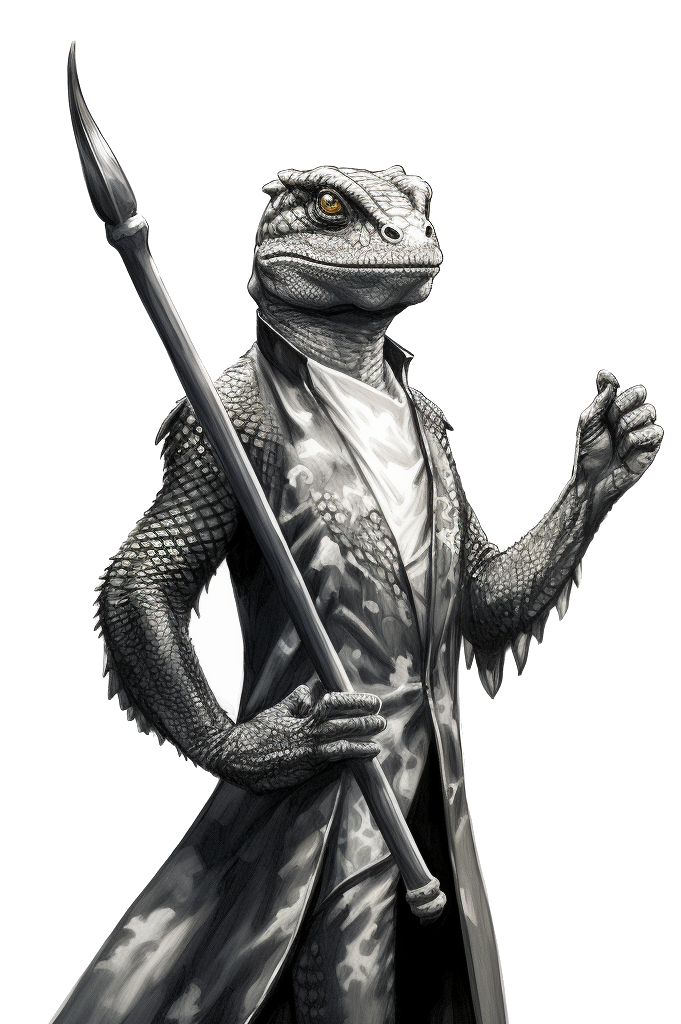
\includegraphics{monsters/Reptiles}
\end{center}

\newpage
\mysubsection{Shades}{monster-order-shades-detail}

\myimage{monsters/Unquiet_Spirit}





\MONSTER[
  NM=Banshee,
  LK=monster-banshee,
  SPD=Base,
  AT=d4 1 Close,
  WK=d12,
  HD=6,
  PR=Average,
  SK=0,
  MR=Orderly,
  SV=6,
  SPL=0,
  TRT=\small{\mytrait{Unhallowed}{monster-trait-unhallowed}; \mytrait{Terrifying}{monster-trait-terrifying}; \mytrait{Spectral}{monster-trait-spectral}; \mytrait{Otherworldly}{monster-trait-otherworldly}},
  ACT=None
 ]
Long lanky hair covers a face you can never seem to make out, a rotting gray cloak over a bottle green dress.  Any Adventurer struck by a Banshee must make an \INSANITY try in addition to the damage taken.

If a Banshee is slain, it will let out an ear-splitting keening - all creatures (Adventurer or Monster alike) must immediately \SAVE{Doom} or fall to 0 Flesh (meaning they must roll their \DEATH at the top of the Moment).

\MONSTER[
  NM=Shadow,
  LK=monster-shadow,
  SPD=Base,
  AT=d10 1 Close,
  WK=d16,
  HD=4,
  PR=Average,
  SK=0,
  MR=Orderly,
  SV=8,
  SPL=0,
  TRT=\small{\mytrait{Unhallowed}{monster-trait-unhallowed}; \mytrait{Terrifying}{monster-trait-terrifying}; \mytrait{Spectral}{monster-trait-spectral}; \mytrait{Otherworldly}{monster-trait-otherworldly}; \mytrait{Bloodthirsty}{monster-trait-bloodthirsty}},
  ACT=None
 ]
Enraged and malicious spirits that lurk in dark corners of crypts and tombs (treat as Invisible while they are hiding under these conditions). Shadows are attracted to injured or bleeding Adventurers, and will try to pick them off first.





\MONSTER[
  NM=Unquiet Spirit,
  LK=monster-unquiet-spirit,
  SPD=Base,
  AT=d4 + Life Drain / 1 Close,
  WK=varies,
  HD=0,
  PR=Weak,
  SK=0,
  MR=Orderly,
  SV=12,
  SPL=0,
  TRT=\mytrait{Unhallowed}{monster-trait-unhallowed}; \mytrait{Terrifying}{monster-trait-terrifying}; \mytrait{Spectral}{monster-trait-spectral}; \mytrait{Otherworldly}{monster-trait-otherworldly},
  ACT=None
 ]


Unquiet spirits sap energy from their victims unless the victim \RBTRY{\FOC}{\FOC}. If the Adventurer fails, roll a d6:


\mynumlist {
    \item Shift your \PRE \DCDOWN.
    \item Shift your \AWA \DCDOWN.
    \item Shift your \CLR \DCDOWN.
    \item Shift your \TAL \DCDOWN.
    \item d4 Damage to Grit.
    \item 1 Damage directly to Flesh (cannot be blocked by Armor).
}


\callout {
Apparition: 1HD, Save d4, Wk d24, Foc: d6
Spook: 3HD, Save d8+1, Wk d20, Foc: d8
Phantom: 5HD, Save d12+2, Wk d16, Foc: d10
Ghost: 7HD, Save d16+3, Wk d10, Foc: d12
}

\newpage

\end{multicols*}
\mysubsection{Swarms}{monster-order-swarms-detail}
\myimage{monsters/Locust}
\begin{multicols*}{2}




\MONSTER[
  NM=Insect Swarm,
  LK=monster-insect-swarm,
  SPD=Base,
  AT=\HD x2 All Close,
  WK=d20,
  HD=0,
  PR=Average,
  SK=0,
  MR=n/a,
  SV=d8+1,
  SPL=0,
  TRT=\mytrait{Mindless}{monster-trait-mindless}; \mytrait{Zoological}{monster-trait-zoological}; \mytrait{Swarming}{monster-trait-swarming},
  ACT=None
 ]
Swarms of carnivorous beetles, biting ants, spiders, etc.

If an Insect Swarm strikes an Adventurer's Flesh, add an additional +2 damage.




\MONSTER[
  NM=Snake Swarm,
  LK=monster-snake-swarm,
  SPD=Base,
  AT=\HD x2 All Close,
  WK=d20,
  HD=0,
  PR=Average,
  SK=0,
  MR=n/a,
  SV=12,
  SPL=0,
  TRT=\mytrait{Mindless}{monster-trait-mindless}; \mytrait{Zoological}{monster-trait-zoological}; \mytrait{Swarming}{monster-trait-swarming},
  ACT=None
 ]
Swarms of venomous snakes of all shapes and kinds.

If a Snake Swarm strikes an Adventurer's Flesh, they must roll a \SAVE{Toxins} or suffer the effects of a Noxious (d6) Toxin.


\MONSTER[
  NM=Vermin Swarm,
  LK=monster-vermin-swarm,
  SPD=Base,
  AT=\HD x2 All Close,
  WK=d20,
  HD=0,
  PR=Average,
  SK=0,
  MR=n/a,
  SV=d8+1,
  SPL=0,
  TRT=\mytrait{Mindless}{monster-trait-mindless}; \mytrait{Zoological}{monster-trait-zoological}; \mytrait{Swarming}{monster-trait-swarming},
  ACT=None
 ]
Swarms of rats, mice, and other carrion feeders. The Swarm will deal 2x\HD of damage to all creatures Close to it (so if you create a 2 \HD swarm, it will deal 4 damage).

If a Vermin Swarm strikes an Adventurer's Flesh, the Adventurer must \SAVE{Toxins} or roll on the \mypg{Diseases}{vulgate-medicine-diseases} table.

\newpage
\mysubsection{Walking Dead}{monster-order-walking-dead-detail}




\MONSTER[
  NM=Lich,
  LK=monster-lich,
  SPD=Base,
  AT=see below,
  WK=d4,
  HD=9,
  PR=Weak,
  SK=0,
  MR=n/a,
  SV=3,
  SPL=0,
  TRT=\mytrait{Mindless}{monster-trait-mindless}; \mytrait{Dead}{monster-trait-dead}; \mytrait{Unhallowed}{monster-trait-unhallowed}; \mytrait{Terrifying}{monster-trait-terrifying}; \mytrait{Otherworldly}{monster-trait-otherworldly},
  ACT=None
 ]
A once-Mortal who has performed the profane right of \mytrait{Lichdom}{occultism-lichdom}. You are encouraged to stat an appropriately leveled Adventurer, but if you're in a pinch, the following should work.

Each ability below has a \UD attached to it.  Using one of these abilities counts as a Combat action:

\mybullet {
    \item  Soulfire (d6): d24+4 damage to d4 Nearby creatures who fail a \\~ \SAVE{Hexes}.
    \item  Level Drain (d4): d4 Nearby creatures must \SAVE{Hexes} or drop all four facets of their \mybold{Personality} \DCDOWN.
    \item  Mangle Flesh (d4): One Nearby creature must \SAVE{Hexes} or reduce their \VIG or \DEX  \DCDOWN (player's choice).
    \item  Ray of Death (d4): One Nearby creature must \SAVE{Hexes} or be reduced to 0 Flesh (and roll their \DEATH at the top of the Moment).
}


Additionally, a Lich is usually armed with a \mypg{Magic Staff}{wonder-staff-magic} or \mypg{Magic Sword}{wonder-sword-magic} of suitable power. 

If a Lich is slain but its phylactery remains intact, it will reform at the next sunset.  If it reforms, all of its \UD and Health reset to normal.

\cbreak

\vspace*{20mm}
\myimage{monsters/Lich}
\newpage

\MONSTER[
  NM=Skeleton,
  LK=monster-skeleton,
  SPD=Base,
  AT=weapon or d4 / 1 Close,
  WK=d24,
  HD=1,
  PR=Average,
  SK=d4,
  MR=n/a,
  SV=11,
  SPL=0,
  TRT=\mytrait{Mindless}{monster-trait-mindless}; \mytrait{Dead}{monster-trait-dead}; \mytrait{Unhallowed}{monster-trait-unhallowed},
  ACT=None
 ]
The classic - skeletal remains of Mortals, bent to unholy purpose. Against Stabbing weapons, skeletons have d4 Soak (otherwise, damage is normal).

\myimage{monsters/Skeleton}





\MONSTER[
  NM=Vampire,
  LK=monster-vampire,
  SPD=Base,
  AT=2d6  1 Close,
  WK=d10,
  HD=7,
  PR=Average,
  SK=0,
  MR=n/a,
  SV=5,
  SPL=3d4,
  TRT=\mytrait{Mindless}{monster-trait-mindless}; \mytrait{Dead}{monster-trait-dead}; \mytrait{Unhallowed}{monster-trait-unhallowed}; \mytrait{Bloodthirsty}{monster-trait-bloodthirsty}; \mytrait{Cannibal}{monster-trait-cannibal},
  ACT=None
 ]


Bloodthirsty fanged walking dead (everyone has an idea of what a vampire looks like, from Nosferatu to Dracula, so go with whatever makes sense for your game).

Once per Combat, in lieu of an attack, the vampire may attempt to charm a Nearby victim.  The victim must make a \SAVE{Hexes} - if they Fail, they immediately fall under the Vampire's sway for \DUR{d6}. A Vampiric Charm is particularly potent, and the victim will fight for the Vampire or willingly allow themselves to be bitten - though they will stop short of taking their own life.

If a Vampire's attack hits Flesh, the victim is affected by \effect{Bleeding}.  The Vampire heals 1 Health at the top of every Moment for every creature Close to it that is Bleeding.

If reduced to 0 Health - and not in a manner appropriate for truly killing vampires in your game - the vampire turns into a cloud of mist and escapes.


\MONSTER[
  NM=Zombie,
  LK=monster-zombie,
  SPD=Slow,
  AT=d8 1 Close,
  WK=d20,
  HD=2,
  PR=Strong,
  SK=0,
  MR=n/a,
  SV=10,
  SPL=0,
  TRT=\mytrait{Mindless}{monster-trait-mindless}; \mytrait{Dead}{monster-trait-dead}; \mytrait{Unhallowed}{monster-trait-unhallowed}; \mytrait{Pack}{monster-trait-pack}; \mytrait{Cannibal}{monster-trait-cannibal},
  ACT=\mytrait{Grapple}{monster-action-grapple}
  ]

Unless they get the Drop on you, you always win Init against a Zombie. 

The initial attack from a Zombie should be treated as a \mypg{Grappling}{monster-action-grapple} attack.  If they succeed, their bite automatically hits during their turn in the following Moments.

\begin{center}
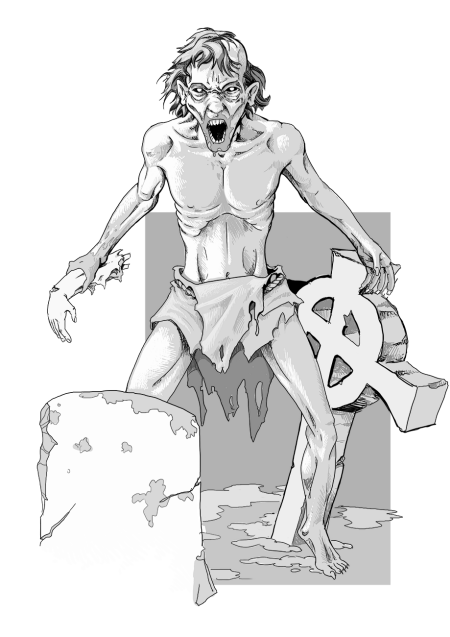
\includegraphics{monsters/Zombie}
\end{center}
\newpage
% MONSTERS END



\mysubsection{Elementals}{monster-elementals}

\callout{
 Elemental Monsters immune to all Arcana except the \mytrait{Secrets of Elements}{arcana-wizardry-secrets}.
}





\MONSTER[
  NM=Lesser Elemental,
  LK=monster-lesser-elemental,
  SPD=Base,
  AT=d6+d8 1 Close,
  WK=d16,
  HD=5,
  PR=Average,
  SK=d4,
  MR=n/a,
  SV=7,
  SPL=0,
  TRT=\mytrait{Otherworldly}{monster-trait-otherworldly},
  ACT=None
]
Lesser elementals come in 6 types: Ice, Blood, Mud, Smoke, Dust, and Clay

\mybullet {
  \item \mybold{Ice} Wind and Water. Ice elementals freeze the ground Close to themselves - anyone who tries an Attack against the elemental while Close must \RSTRY{\DEX} after their attack (hit or miss) or fall Prone.

  \item \mybold{Blood} Water and Fire.  If a Blood elemental attack hits Flesh, it heals for a number of points equal to the amount of Flesh damaged.

  \item \mybold{Mud} Earth and Water.  The ground near the Mud elemental turns to knee deep muck.  Anyone Close to the elemental cannot move without a successful \RSTRY{\VIG}.

  \item \mybold{Smoke} Fire and Wind.  When a Smoke elemental is struck the first time in Combat, roll a d4 - this number of illusory Smoke elementals appear around it.  The illusions have only 1 Health, but any attack hits one of these illusions first (area of effect spells can potentially wipe them all out).

  \item \mybold{Dust} Wind and Earth.  Each time a Dust Elemental is struck by a Close physical attack, the attacker must roll a \SAVE{Doom} or be \effect{Blinded} for \DUR{d4}.

  \item \mybold{Clay} Earth and Fire.  Whenever a Clay elemental is struck by a weapon, the attacker must \RSTRY{\VIG} or their weapon is stuck in the Clay elemental, and cannot be freed until the creature is slain.
}

\begin{center}
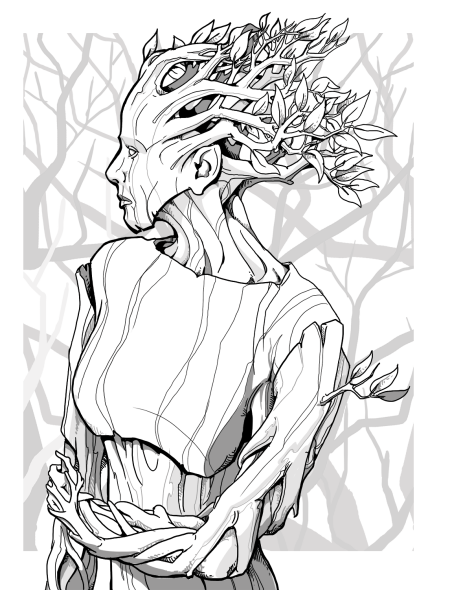
\includegraphics{monsters/Elemental_1}
\end{center}

\MONSTER[
  NM=Greater Elemental,
  LK=monster-greater-elemental,
  SPD=Base,
  AT=d20 1 Close,
  WK=d10,
  HD=7,
  PR=Strong,
  SK=d8,
  MR=n/a,
  SV=5,
  SPL=0,
  TRT=\mytrait{Otherworldly}{monster-trait-otherworldly},
  ACT=None
]
Greater elementals come in 4 types: Water, Wind, Fire, and Earth.  Each one has their own set of Abilities.

\mybullet {
  \item \mybold{Water Elementals} have the \mytrait{Splitting}{monster-trait-splitting} Trait. Immune to damage from Stabbing weapons. They automatically win \RB : \FOC tries.

  \item \mybold{Wind Elementals} have the \mytrait{Amorphous}{monster-trait-amorphous} and \mytrait{Twitchy}{monster-trait-twitchy} Traits. Immune to damage from Bashing weapons. They automatically win \RB : \DEX tries.

  \item \mybold{Fire Elementals} have the \mytrait{Berserk}{monster-trait-berserk} and \mytrait{Frenzied}{monster-trait-frenzied} Traits. When struck by a Fire Elemental, the Adventurer must roll a \SAVE{Doom} or become \effect{Enflamed}. Fire Elementals automatically win \RB : \INT tries.

  \item \mybold{Earth Elementals} have the \mytrait{Strong}{monster-trait-strong} Trait.  They can pick up and throw an Adventurer 30m. Earth Elementals automatically win \RB : \VIG tries.

}


\newpage



\mysubsection{Dragons}{monster-dragons}

\begin{center}
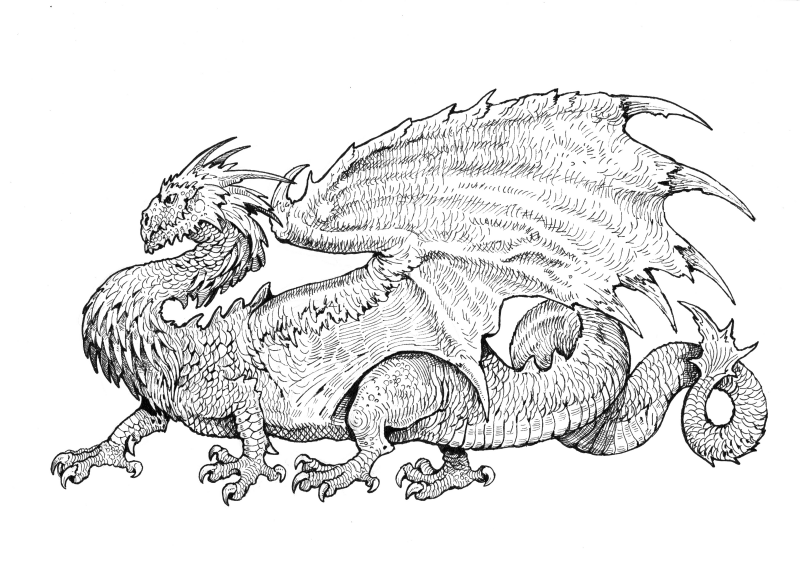
\includegraphics{monsters/Dragon1}
\end{center}


\MONSTER[
  NM=Dragon,
  LK=monster-dragon,
  SPD=Base,
  AT=d20 1 Close,
  WK=d10,
  HD=7,
  PR=Strong,
  SK=d6,
  MR=n/a,
  SV=5,
  SPL=0,
  TRT=\mytrait{Otherworldly}{monster-trait-otherworldly},
  ACT=\mytrait{Rage}{monster-action-rage};  \mytrait{Trample}{monster-action-trample}
]

\callout {
    Dragons are immune to \mypg{Secrets of the Mind}{arcana-wizardry-secrets}.

    Dragons are immune to damage from their elemental type (see below).

    Dragons automatically win \myital{any} \RB tries.
}


\myhighlight{Creating a Dragon}{monster-dragon-creation}

\mybold{Step 1}

\callout {
Roll 3d6:
    \mynumlist {
      \item First d6 is the dragon's color (elemental type): 1) Red, 2) Black, 3) White, 4) Blue, 5) Green, 6) Bone
      \item Second d6 is the dragon's size: 1) Small, 2) Middling, 3) Large, 4) Huge, 5) Colossal, 6) Titanic
      \item Third d6 is the dragon's age: 1) Juvenile, 2) Adult, 3) Old, 4) Very Old, 5) Ancient, 6) Wyrm
    }
}

\cbreak

\mybold{Step 2}

\callout {
Roll a d6 a number of times equal to the dragon's \mybold{size}.  Results stack:

    \mytable{l X}{
    \thead{d6} & \thead{Modification}  \\
    }{
        1 & Increase Damage 1 Tier \\
        2 & Increase Weakness 1 Tier \\
        3 & Increase Soak 1 Tier \\
        4 & Increase \HD 1 Tier \\  
        5 & Increase Spell Dice 1 Tier \\
        6 & Increase Breath Weapon +d6 \\
    }
}

\mybold{Step 3}

Roll a d6 a number of times equal to the dragon's \mybold{age}.  Results \myital{do not} stack. If you get the same roll, roll again i.e. a Wyrm will have all of these enhancements. Enhancements are explained on the next page:

  \mytable{l X}{
    \thead{d6} & \thead{Enhancement}  \\
  }{
    1 & Wing Buffet \\
    2 & Tail Slap \\
    3 & Spell Resistance \\
    4 & Terrifying Presence \\  
    5 & Roar \\
    6 & Flight \\
  }

\mybold{Step 4}

Finally, take the \SUM of the dragon's age and size rolls.  This is the base damage for their breath weapon, as well as how many times they can use it per Session.

\newpage

\end{multicols*}

\myhighlight{Tiers}{dragon-tiers}

  \mytable{X c c c c c}{
    \thead{Tier} & \thead{Damage} & \thead{Weakness} & \thead{Soak} & \thead{Hit Dice} & \thead {Spell Dice\Asterisk} \\
  }{
    Tier 0 & d20 1 Close & d10 & d6 & 7 & 0 \\
    Tier 1 & d24 1 Close & d8 & d8 & d8 & 2 \\ 
    Tier 2 & d20+4 1 Close & d6 & d10 & 11 & 4 \\
    Tier 3 & d24+4 1 Close & d4 & d12 & 13 & 6 \\
    Tier 4 & d24+6 1 Close & d3 & d16 & 15 & 8 \\
    Tier 5 & d24+8 1 Close & d2 & d20 & 17 & 10 \\
    Tier 6 & d24+10 1 Close & 0 & d24 & 19 & 12 \\
  }

\footnotesize \Asterisk Dragons use their Spell Dice to invoke \mypg{Secrets}{arcana-wizardry-secrets}, etched in their skulls. They can invoke a number of Secrets equal to their Spell Dice.
\normalsize


\myhighlight{Enhancements}{dragon-enhancements}

\mybold{Wing Buffet} :  The Dragon can buffet its wings against All Close (Distinct) Adventurers.  If struck, the Adventurer takes d6 damage.  They must \RS : \VIG or \DEX (player choice) or be moved somewhere Nearby.


\mybold{Tail slap:} The dragon can slap with its tail against All Close (Distinct) Adventurers.  If struck, the Adventurer takes d10 damage and must \RSTRY{\DEX} or be knocked \effect{Prone}.


\mybold{Spell resistance:}   The dragon is not affected by spells on a 2-in-6 (this is separate from their Save).


\mybold{Terrifying Presence:}   Creatures with fewer than half the dragon's \HD (rounded down) must \SAVE{Doom} or become \effect{Afraid}.  Seeing this creature the first time prompts an \INSANITY try.


\mybold{Roar:}  In lieu of attacking, the dragon can let out a horrifying roar.  Every creature Far-Away or closer must make a \SAVE{Doom} or become \effect{Deafened} for \DUR{d4}.
 

\mybold{Flight:}  The dragon has the Trait \mytrait{Flying}{monster-trait-flying}. The dragon can choose to use its breath weapon while in the air.

\begin{center}
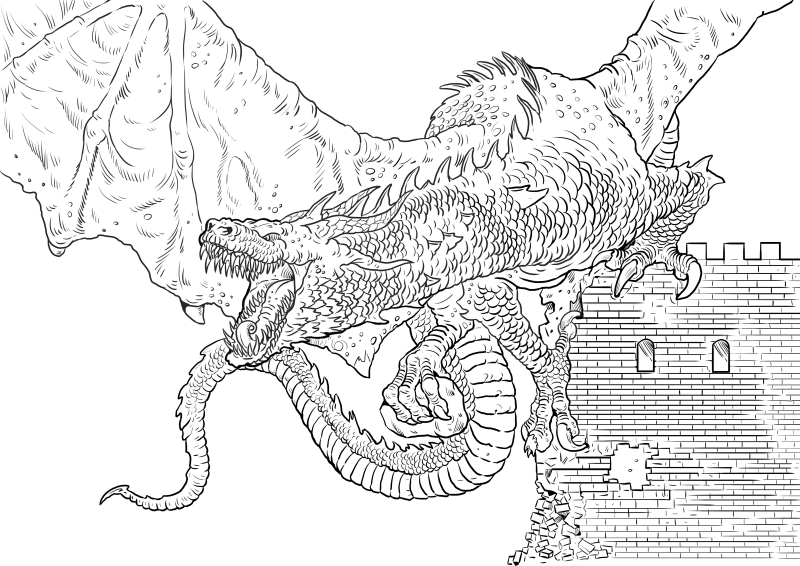
\includegraphics{monsters/Dragon2}
\end{center}

\newpage

\begin{multicols*}{2}

\myhighlight{Breath Weapon}{dragon-breath-weapon}

  \mytable{c c c X}{
    \thead{\SUM Age+Size} & \thead{Damage} & \thead{Uses} & \\
  }{
    2-4 & 6d6 & 1 & \\
    5-7 & 7d6 & 1 & \\
    8-10 & 8d6 & 2 & \\
    11 & 9d6 & 2 & \\  
    12 & 10d6 & 3 & \\
  }

Note that a dragon's breath weapon affects all Close OR Nearby (Distinct) Adventurers, and hits automatically. 

There are 2 ways to reduce the damage from a breath weapon:
\mybullet {
  \item Make a \RSTRY{\TAL}. If you don't roll a Failure, take half damage.
  \item Make a \SAVE{Doom}. If you succeed, take half damage again.
}

These effects stack - so making your \RS:\TAL try and a \SAVE{Doom} will reduce the amount of damage by 75\%. Roll the check and Save before you apply damage.

The color of the dragon also affects the breath weapon type:


\cbreak

\mybold{Red:}   Fire.  \RS:\TAL. If you fail, you become \effect{Enflamed}.

\mybold{Black:}  Acid.  If the attack hits Flesh, take 2d4 acid damage for 2d4 Moments.

\mybold{White:} Frost. \SAVE{Doom} or take \DCDOWN damage to a single facet of your \mybold{Identity} (your choice).

\mybold{Blue:}  Lightning.  If you're wearing metal armor, take an additional 2 points of damage per die.

\mybold{Green:}  Corrosive gas.  Everyone must try their Armor \UD 3 times.

\mybold{Bone:}  Void.  \SAVE{Doom} or take \DCDOWN damage to a single facet of your \mybold{Personality} (your choice).

\mybold{You can sunder your shield to prevent the secondary effect (but not the damage).}


